\documentclass[12pt]{article}

% for footnotes
\makeatletter
\newcommand\footnoteref[1]{\protected@xdef\@thefnmark{\ref{#1}}\@footnotemark}
\makeatother

\usepackage{common}
\usepackage{macros}
\usepackage{nameref}
\usepackage{pdflscape}

\title{HW1: Classification}
\author{Jiafeng Chen \and
Francisco Rivera}
\begin{document}

\maketitle{}
\section{Introduction}
In this write-up, our main focus is language modeling. That is, given words in a
sentence, can we predict the word that follows? We implemented a trigram model,
a embedding neural network model, an LSTM, and a few extensions---including
warm-starting from pre-trained embeddings, ensemble models, and multi-head
attention decoder. 

\section{Problem Description}

The focus of the problem set is language modeling. We start with sequences of
words $w \in \mcV$ in some vocabulary $\mcV$ and aim to predict the last word in
the sequence which we cannot observe. We can do this probabilistically by
attempting to estimate,
\begin{equation}
\label{eq:cond_prob}
    p(w_i \mid w_1, \ldots, w_{i-1})
\end{equation}
that is, the conditional distribution over the last word conditional on the
words leading up to it.

In particular, there will be a special word, $w_\text{unk} \in \mcV$ which
represent an unknown word; we use this whenever we encounter a token we had not
previously seen in training. 

In some models, we represent words with dense embeddings. That is, each word
gets assigned a vector $\boldv \in \mathbb{R}^d$ where $d$ is the embedding
dimension. These embeddings are trained as part of the model, but can also be
initialized to pre-trained values.

\section{Model and Algorithms}

\subsection{Neural Network Language Model}
\label{sub:nnlm}
Following \cite{bengio2003neural}, we implement a neural network language model
(NNLM). We model \eqref{eq:cond_prob} by first assuming limited dependence: \[
p(w_i \mid w_1,\ldots,w_{i-1}) = p(w_i \mid w_{i-1}, \ldots, w_{i-k}),
\]
i.e., the current word only depends on the past $k$ words, a useful restriction
motivated by n-gram models. Next, we convert input tokens $w_{i-1},\ldots,w_
{i-k}$ into embedding vectors $\br{\boldv_{i-t}}_{t=1}^k$ and concatenate them
into a $dk$ vector $\bm v_{i-k:i-1}$. We then pass this vector into a
multilayer perceptron network with a softmax output into $|\mathcal V|$ classes.
We implement this efficiently across a batch by using a convolution operation,
since convolution acts like a moving window of size $k$. This way we can
generate $T - k + 1$ predictions for a sentence of length $T$. We depict the
convolution trick in \Cref{fig:nnlm}. 

\begin{figure}[tb]
    \centering
    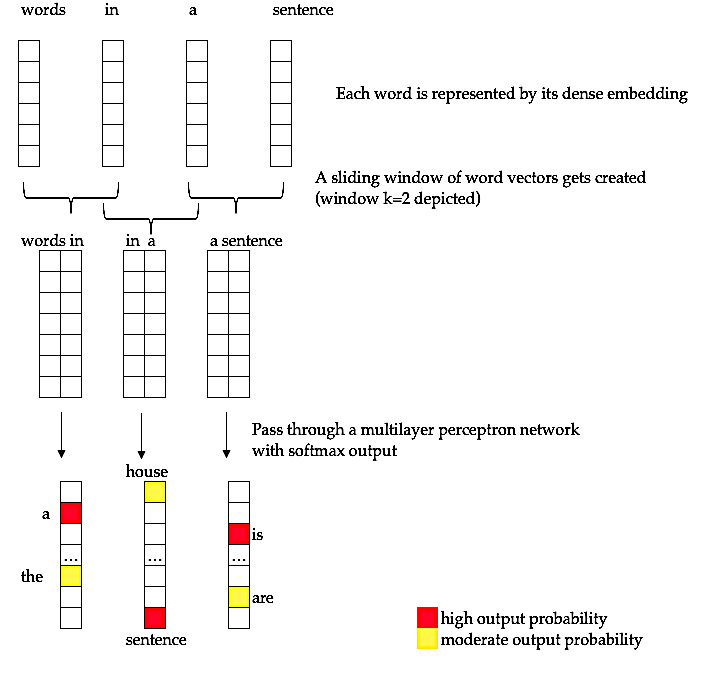
\includegraphics[width=.7\textwidth]{figs/nnlang.png}
    \caption{Diagram for \Cref{sub:nnlm}}
    \label{fig:nnlm}
\end{figure}

\subsection{Multihead Attention}
\label{sub:attn}

Following \cite{vaswani2017attention}, we implement a variant of the multi-head
attention
decoder network. Instead of passing the last hidden state from an LSTM $h_t$ to
predict $h_{t+1}$, we use a concatenation of $h_t$ and a \emph{context vector}
$c_t = a_1 h_1 + \cdots + a_{t-1} h_{t-1}$ for \emph{attention values}
$a_1,\ldots, a_{t-1}$ residing in the unit simplex. Following 
\cite{vaswani2017attention}, we use the \emph{scaled attention} mechanism,
where \[
\bm a = \softmax\pr{\br{\frac{h_i^T h_t}{\sqrt{\dim(h_t)}}}_{i=1}^{t-1}}.
\]
In \emph{multi-head attention}, we repeat the attention mechanism above on
different linear projections of $h_1,\ldots,h_t$, with the motivation being that
we wish to capture similarity on different projections of words---one attention
layer could be capturing grammar, another semantics, a third pronoun
association, etc. We depict the architecture in \Cref{fig:attn}, for $t=3$ and
predicting $t+1$.
\begin{figure}[tb]
    \centering
    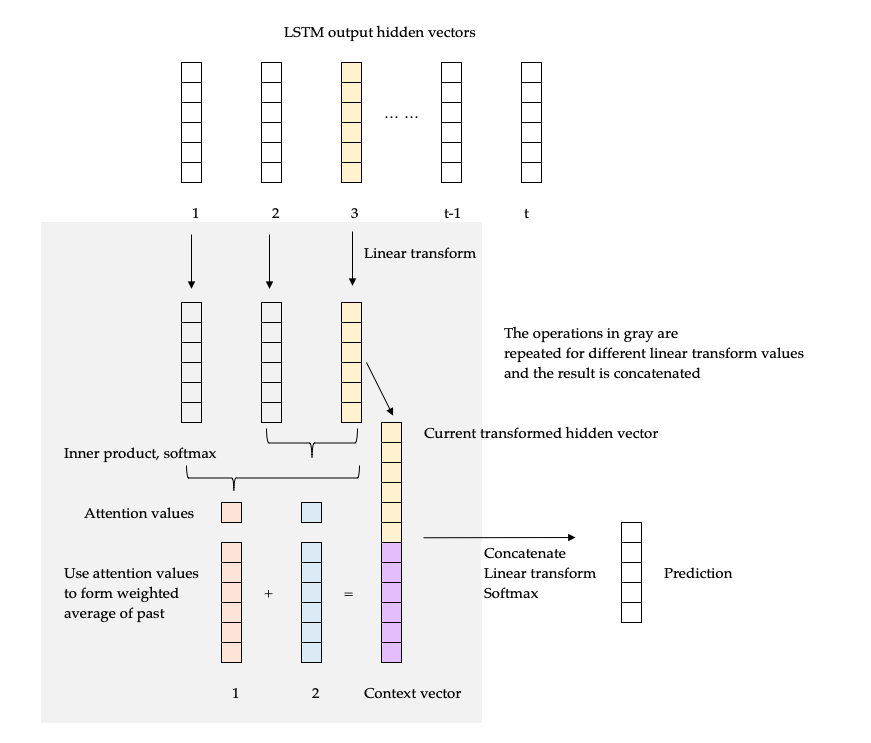
\includegraphics[width=\textwidth]{figs/attention.png}
    \caption{Diagram for \Cref{sub:attn}. In this diagram, we predict the
    fourht word in the sentence by conditioning on the first three. We compute
    attention values of $h_3$ with $h_2$ and $h_1$ and concatenate $h_3$ with a
    context vector $a_1 h_1 + a_2 h_2$, where $a_i$ are the attention values.
    We pass the resulting vector through a linear transformation and softmax
    output.
    In multi-head attention, we repeat the process for different projections of
    $h_1,h_2,h_3$ and
    concatenate the results. }
    \label{fig:attn}
\end{figure}

Certain computational tricks need to be employed for efficient utilization of
the GPU. Unlike the encoding attention network, the decoder cannot condition on
future information when predicting the future. As a result, each attention layer
can only look at past hidden states. We parallelize the procedure and take
advantage of GPU hardware by applying attention as usual, computing every
inner product $h_i^T h_j$ for all $i,j$, and use a mask that sets entries with
$h_i^T h_j$
to $-\infty$ if $j \le i$ (which correspond to the forbidden attention
links by looking ahead) before applying the softmax. 
\section{Experiments}
\section{Conclusion}


\bibliographystyle{apalike}
\bibliography{writeup}

\end{document}
